\documentclass[11pt, letterpaper, oneside]{article}

% This document is a simple latex template for reports. It follows the official Lab9K Styleguide, https://github.com/lab9k/Styleguide.

% Packages

\usepackage[dutch]{babel}

\usepackage{fontspec}               % Use own font

\usepackage{geometry}               % Interface to change page dimensions
\usepackage{parskip}                % For better spacing and indenting of paragraphs

\usepackage{graphicx}               % Images
\usepackage[export]{adjustbox}				% Wrap text around figures
\usepackage{fancyhdr}               % Headers and footers
\usepackage{caption}                % Caption

\usepackage{sectsty}                % Manipulate fonts of various sectional headings
\usepackage{enumitem}               % Manipulate enumerate, mdwlist and paralist
\usepackage{makecell}               % Improved tabular layout

\usepackage{url}
\usepackage{hyperref}

\usepackage{anyfontsize}            % Specify font sizes
\usepackage{xcolor}                 % Define own colours

\usepackage{lipsum}                 % Lorem ipsum

%\usepackage{minted}				% For code snippets

% Configure content of title page

\title{Rapport \\ Chatbot Gentse Feesten 2018}
\author{}
\newcommand{\organisation}{Lab9K}
\newcommand{\promotor}{Hans Fraiponts}
\newcommand{\subject}{Rapport Chatbot Gentse Feesten 2018}
\date{23 juli 2018}

% Colour scheme (based on logo)

\definecolor{priColour}{HTML}{026495}              % primary colour
\definecolor{secColour}{HTML}{4a92b8}              % secondary colour

% General configuration and package setup

\geometry{}
\graphicspath{ {figuren/} }    % Map containing all images
\setlength{\headheight}{15pt}

\makeatletter \hypersetup{
	pdfauthor = {\@author},
	pdftitle = {\@title},
	pdfsubject = {\subject},
	colorlinks=true,
	linkcolor=priColour,
	filecolor=priColour,  
	urlcolor=priColour
}

% Fonts

\setmainfont{Ubuntu}
\setmonofont{Ubuntu}

% General styling

% Use the primary colour for all titles
\sectionfont{\color{priColour}}
\subsectionfont{\color{priColour}}
\subsubsectionfont{\color{priColour}}

% Header
\pagestyle{fancy}
\renewcommand{\headrulewidth}{0pt}
\rhead{\@date}

\begin{document}
	% TITEL %
	\begin{figure}
			
\includegraphics[width=0.27\textwidth,keepaspectratio]{figuren/logo} % Logo of Lab9K
	\end{figure}
	\vspace*{0.35cm}
	
	\noindent
	\fontsize{30pt}{28pt}\selectfont\textcolor{priColour}{\textbf{\@title}}\newline
	
	\fontsize{11pt}{15pt}\selectfont
	
	% BODY %
	
	\section{Statistieken}
	
	Dagelijks maakten enkele tientallen gebruikers gebruik van de chatbot. In totaal waren er een goede 250 gebruikers.

	\begin{figure}[h]
		\centering
		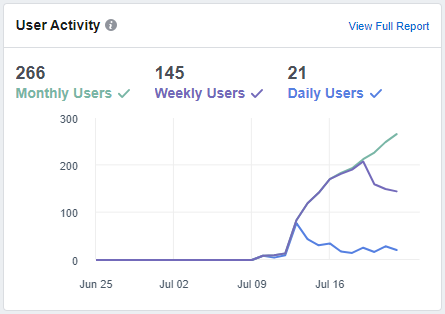
\includegraphics[width=0.7\linewidth]{./figuren/user-activity}
		\caption{Algemene User Activity}
		\label{user-activity}
	\end{figure}

	\clearpage

	De user retention lag echter wel laag. Veel mensen maakten slechts éénmaal gebruik van de chatbot.
	
	\begin{figure}[h]
		\centering
		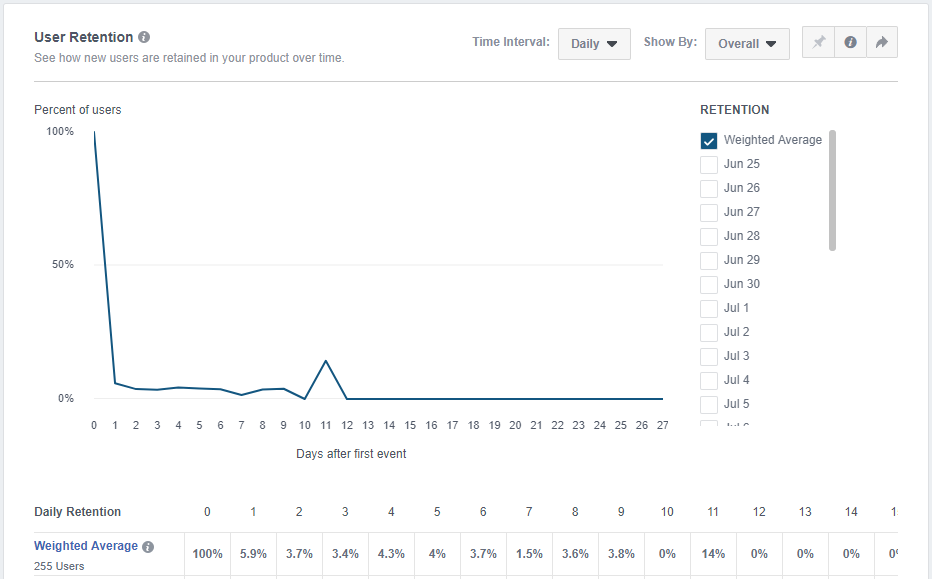
\includegraphics[width=0.7\linewidth]{./figuren/user-retention}
		\caption{User Retention}
		\label{user-retention}
	\end{figure}

	Tenslotte hieronder nog enkele verdere statistieken in verband met de user base.
	
	\begin{figure}[h]
		\centering
		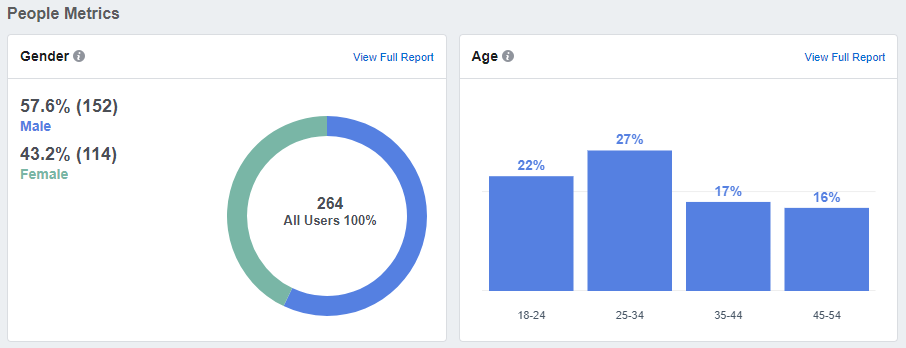
\includegraphics[width=0.7\linewidth]{./figuren/people-metrics}
		\caption{People Metrics}
		\label{people-metrics}
	\end{figure}

	\clearpage
	
	\section{Ontvangen Feedback}
	
	Gebruikers konden feedback naar de chatbot sturen. Ze konden zeggen of ze tevreden, neutraal of niet tevreden waren en konden eventueel wat commentaar achterlaten.
	
	In totaal kregen we 4 keer een \textit{Tevreden}, 3 keer een \textit{Neutraal} en 6 keer een \textit{Niet Tevreden}.
	
	Eén van de commentaren was "Krijg geen antwoord op mijn vraag waar Willy Bart  op treedt tijdens de Gentse feesten". Als mensen dus vragen naar een bepaalde groep of een bepaald evenement kon de chatbot hier niet op antwoorden. Dit zou opgelost kunnen worden door namen van zangers of namen van evenementen te herkennen in vragen (aan de hand van entities in Dialogflow).
	
	Een ander commentaar was "Ik wil praten tegen een echt persoon". Vaak kon de chatbot niet antwoorden op een bepaalde vraag. De chatbot geeft dan een \textit{default fallback}. Sommige mensen beëindigden dan de conversatie. Andere mensen probeerden dan hun vraag anders te formuleren. Soms kon de bot dan wel succesvol antwoorden, maar vaak lukte dit niet. Op zulke momenten zou het misschien handig zijn om een verantwoordelijke voor de Gentse Feesten manueel te laten antwoorden. Dit zou kunnen gebeuren door rechtstreeks via Facebook een bericht te sturen vanuit de pagina van de Gentse Feesten. Een andere mogelijkheid is om de chatbot te laten vragen voor het e-mailadres van de gebruiker. Er kan dan via de backend een mail verstuurd worden naar een verantwoordelijke en deze kan dan via mail de vraag beantwoorden.
	
	\clearpage
	
	\section{Verdere Observaties}
	
	Facebook laat toe om alle conversaties met de bot rechtstreeks te bekijken. We hebben de meeste conversaties overlopen en hebben hierbij enkele dingen vastgesteld.
	
	Heel veel mensen sturen een bericht in verband met verloren voorwerpen naar de chatbot. De chatbot kon hier meestal correct op antwoorden met een doorverwijzing naar de politie. Dit zou misschien verbeterd kunnen worden door een specifieker antwoord te geven. De chatbot zou bijvoorbeeld rechtstreeks kunnen doorverwijzen naar een verantwoordelijke voor een bepaald feestplein.
	
	Er waren heel wat vragen in verband met foto's. Enerzijds waren er een aantal fotografen die vroegen of ze ergens hun foto's konden publiceren. Anderzijds vroegen sommige mensen waar ze foto's konden vinden van een bepaald plein op een bepaalde dag. Iets anders wat we opmerkten is dat veel mensen spontaan foto's sturen naar de chatbot.
	
	De chatbot kreeg vaak zeer lange berichten binnen. Een aantal mensen stuurden een soort van formele e-mail, een bericht met begroeting en vaak ook in verschillende talen. \\ Hier reageerde de chatbot nooit op, zelf niet met een \textit{default fallback}. Het was precies alsof de chatbot deze lange berichten gewoon negeerde. Na wat verder te testen blijkt dat Dialogflow geen berichten langer dan 256 karakters verwerkt. Er wordt geen enkele foutboodschap opgegooid, berichten langer dan 256 karakters worden gewoonweg genegeerd door Dialogflow.
	
	Er waren een aantal mensen die aan de chatbot vroegen om een bepaalde persoon te vinden die ze waren tegengekomen op de Gentse Feesten.
	
	Heel wat muziekgroepen stuurden de vraag naar de chatbot om op te treden op de Gentse Feesten. De chatbot kon hier een op antwoorden met een doorverwijzing naar de website van de Gentse Feesten waar er men meer info hierover kon vinden. Een verbetering zou misschien zijn om hierbij een verantwoordelijke te laten antwoorden die hun direct beter zou kunnen helpen. Dit zou kunnen op de manieren die hierboven beschreven werden.
	

\end{document}